\documentclass[]{sigplanconf}
\usepackage{stmaryrd}
\usepackage{listings}
\usepackage{multirow}
\usepackage{array}
\usepackage{subfig}
%\usepackage{algorithmic}
\usepackage{algorithm}
\usepackage{algpseudocode}
\usepackage{amsmath}
\usepackage{xfrac}
%\usepackage{amsthm}
\usepackage{amssymb}
\usepackage{xspace}
%\usepackage[pdftex]{graphicx}
\usepackage{graphicx}
\usepackage{siunitx}
\usepackage[svgnames,table]{xcolor}
\usepackage{natbib}
\usepackage{adjustbox}
\usepackage{tabularx}
\usepackage{booktabs}
\usepackage{placeins}
\usepackage{hyperref}
\usepackage{tikz}
\usepackage{subfig,epstopdf, todonotes}
\usetikzlibrary{automata,positioning}
%\usepackage{amsmath,amsfonts,amssymb,mathtools,url,cite,xspace,graphicx,color,stmaryrd,multirow,verbatim,listings,tikz,pspicture,epstopdf,algorithm,listings,algorithmicx,algorithm,caption,todonotes,algpseudocode}
\hypersetup{
    colorlinks,
	linkcolor={blue!50!black},
	citecolor={blue!50!black},
	urlcolor={blue!80!black}
}
\urlstyle{same}

%\newcommand\comment[1]{\ding{110}\ding{43}\textcolor{red}{#1}}

%\newcommand\code[1]{\textsf{\small #1}}
%\DeclareCaptionType{copyrightbox}
\newcommand\sius[1]{\num[group-separator = {,}]{#1}\si{\micro\second}}
\newcommand\sims[1]{\num[group-separator = {,}]{#1}\si{\milli\second}}
\newcommand\sins[1]{\num[group-separator = {,}]{#1}\si{\nano\second}}
\newcommand\tuple[1]{\langle #1 \rangle}
\providecommand{\abs}[1]{\lvert#1\rvert}

%\newcommand{\mc}[3]{\multicolumn{#1}{#2}{#3}}

\begin{document}

\title{Mining timed regular expressions from system traces}

\authorinfo{Greta Cutulenco, Yogi Joshi, Apurva Narayan, and Sebastian Fischmeister}
		   {University of Waterloo, ON, Canada}
		   {\{gcutulen, y2joshi, apurva.narayan, sfischme\}@uwaterloo.ca}

\maketitle


\begin{abstract}

Dynamic behavior of a program can be assessed through an examination of events emitted by the program during execution. For the behavior to be correct it must satisfy a set of specified temporal properties. Temporal properties define the order of occurrence and timing constraints on event occurrence. Such specifications are important for safety-critical real-time systems for which a delayed response to an emitted event may lead to a fault in the system. Since temporal properties are rarely specified for programs and due to the complexity of the formalisms, temporal properties are automatically extracted from traces of program execution. We propose a framework for automatically mining properties that are in the form of timed regular expressions (TREs) from system traces. Using an abstract structure of the property the framework constructs a finite state machine (FSM) to serve as an acceptor. We evaluate our technique on real-world datasets. We formally demonstrate the scalability and performance of our approach by running our implementations on synthesized traces of different sizes with different parameter values.

\end{abstract}

\section{Introduction}
%% author: AN
Temporal behavior of programs has been extensively studied~\cite{lamport1978time, dwyer1999patterns}. Recently, the idea of mining system traces to derive likely temporal specifications of programs has become popular~\cite{lemieux2015general}. Mining techniques generally identify a set of specifications which are satisfied by traces w.r.t. certain criteria. Commonly used patterns of specifications are provided for mining a systems' specifications. Many programs lack formal temporal specifications, and mined specifications are therefore valuable and could be used for a wide variety of activities in software development life cycle (SDLC). These activities include software testing~\cite{dallmeier2010generating}, automated program verification~\cite{kincaid2015automated}, anomaly detection~\cite{christodorescu2008mining}, debugging~\cite{gabel2010online}, etc. Further, mined specifications can assist automated verification techniques because they provide an easy and user-friendly way to describe programs' specifications. As argued by Ammons et al.~\cite{DBLP:conf/popl/AmmonsBL02}, automated verification techniques are unlikely to be widely adopted unless cheaper and easier ways of formulating specifications are developed. Consequently, specification mining has gained significant attention in recent times. Different techniques have been developed for mining specifications using templates expressed using regular expressions, LTL and other custom formats.

Most of the existing research in the context of mining temporal specifications focuses on qualitative notion of time, i.e., the specifications describe an \emph{ordering} of events. For example, an LTL specification $\Box(\mathrm{request}\,\rightarrow\,\lozenge \mathrm{response})$ specifies that a \emph{request} event should always be eventually followed by a \emph{response} event. Most state-of-the-art techniques do not take into account a \emph{quantitative} notion of time, i.e., the actual duration of time between events is not considered. For safety-critical real-time systems, it is important to develop techniques, which allow mining of specifications that account for the quantitative notion of time. For example, mining specifications of interrupt handlers, which complete their executions within a set of predefined deadlines for a real-time system, involves consideration about the quantitative notion of time. Such specifications are of important for safety-critical real-time systems for which a delayed response to an emitted event may lead to a fault in the system. Certain specifications of real-time systems can be modeled using timed regular expressions, which can be in turn translated into the corresponding timed automata.

With a motivation to address the problem of mining specifications with explicit notion of time, we propose a technique to mine instances of timed regular expression (TRE)~\cite{timedregex} templates satisfied by a given system's traces. TREs extend regular expressions by providing additional operators to specify timing constraints between events. By using a set of commonly used patterns of specifications for LTL and regular expressions, we develop the corresponding patterns for TREs. Further, we use the method proposed by Asarin et al. \cite{timedregex} to synthesize the timed automaton for a given TRE. Such timed automaton is then used as a checker to verify whether traces satisfy the corresponding TRE. TRE templates replace actual events in a TRE instance by a variable, which can be assigned a value of an actual event in traces. We provide two algorithms for mining instances of TREs from their templates. Both algorithms require a TRE template and a system's traces as input. The algorithms then use the distinct events in the traces to generate different possible \emph{permutations} of the events that can be formed by substituting the actual events into the variables in the TRE template. Intuitively, the given trace is processed against every permutation to check whether the trace satisfies TRE instances denoted by the corresponding permutations. Further, we define \emph{support} and \emph{confidence} as metrics to evaluate the degree to which a TRE instance is satisfied by a trace. The algorithms then report the permutations which satisfy the given threshold values of support and confidence.

The first algorithm is designed for TRE templates containing negation operator. The second algorithm processes TRE templates without a negation operator. We later prove that although both algorithms' execution times are exponential in terms of the number of variables in individual TRE templates, the second algorithm generally runs faster than the first by a certain factor which depends upon the number of distinct events in a trace and the number of variables in a given TRE template. We also prove that our technique is sound, i.e., a mined specification reported by our algorithms actually satisfies the given thresholds of support and confidence on the provided input traces. Also, our technique is complete, i.e., our algorithms report all TRE instances which comply on given traces w.r.t. the thresholds of support and confidence.

We evaluate our technique on real-world datasets which consist of logs produced by QNX realtime RTOS  \cite{QNX_RTOS} during various runs of application software on different hardware platforms and controller area network (CAN) \cite{CAN}traces of an automobile. We report the performance of our algorithms in terms of the execution time. We demonstrate the scalability and performance of our approach by running our implementations on synthesized traces of different sizes with different values of parameters such as the number of distinct events, the total number of events in traces and the complexity of TRE templates.

In this paper we propose a framework to automatically mine properties that are in the form of timed regular expressions from system traces. Using an abstract structure of the property the framework constructs a finite state machine (FSM) to serve as an acceptor. We encode the concrete properties in a set of matrices. The FSM is used to evaluate the satisfaction of every potential concrete property in the trace. Using a ranking system we infer the strongest concrete properties that describe the system and thus deduce a set of interesting system specifications.

The key contributions of this paper involve developing an efficient framework for extracting complex temporal properties that take on the form of timed regular expressions and evaluating the framework experimentally on industrial real-time systems:

\begin{itemize}
\item We develop two novel algorithms to mine instances of timed regular expressions satisfied by a given system's traces. To our knowledge, this is the first technique for mining specifications with explicit notion of timing constraints (Section ~\ref{Approach}),
\item Identifying computational approaches that optimize the extraction of the specified properties (Section ~\ref{Approach}),
\item Demonstrating the frameworks' applicability to large traces collected from real industrial systems  (Section ~\ref{discussion}).
\end{itemize}

\section{Background} \label{Background}

\subsection{Timed Regular Expressions}

Classical automata theory handles only the \emph{qualitative} notion of time, i.e. a sequence of events specifies the ordering of events but not the time between occurrence of these events in terms of ``real time". An abstraction of this sort has been found useful for analysis of certain systems [???], whereas many other application domains require more detailed models which include accurate timing information [???]. For example, we might want to modify a formal specification \emph{``a is followed by b"} to a more precise specification with timing constraints \emph{``a is followed by b within $x$ seconds"}. Since our focus lies on real-time safety-critical systems, we need to develop techniques for mining specifications that include the relevant timing information. We use the formalism of Timed Regular Expressions for our purpose as it allows for defining explicit timing constraints in the model. We will formally describe our nomenclature.

\newtheorem{defns}{Definition}

\begin{defns}[Trace and event]
The alphabet of events is a finite alphabet of strings. An timed sequence of events is a trace.
\end{defns}

The sequences of events in the trace are ordered by time stamps.
The alphabet of events is defined by the system generating the traces. The events have associated meaning pertaining to the functionality of the system.


\begin{defns}[Timed Regular Expression (TRE) \cite{timedregex}]
Timed regular expressions (TREs) over an alphabet $\Sigma$ (also referred to as $\Sigma$-expressions) are defined using the following families of rules:
\begin{itemize}
  \item  \underbar{a} for every letter a $\in \Sigma$ and the special symbol $\epsilon$ are expressions,
  \item If $\varphi$, $\varphi_1$ and $\varphi_2$ are $\Sigma$-expressions and $I$ is an integer bound interval then $\langle \varphi \rangle_I$, $\varphi_1 \dot \varphi_2$, $\varphi_1 \vee \varphi_2$ and $\varphi^*$ are $\Sigma$-expressions.
\end{itemize}
\end{defns}

The novel features here with respect to untimed regular expressions are the meaning of the atom $\underline{\alpha}$ which represents an arbitrary passage of time followed by an event $\alpha$ and the $\textless \phi \textgreater _I$ operator which restricts the metric length of the time-event sequences in [[$\phi$]] to be in the interval I. It is important to note that we use TREs, as defined above, to provide specification templates.


\begin{defns}[TRE Templates]
A TRE template is a TRE in which all of the atomic propositions are either event variables, events, or time intervals.
\end{defns}

A TRE template is a template for the specifications that we want to mine. We use the term \emph{event variable} to denote a place holder for an event. For example, the TRE template $<0.1>[x,y]$ represents \emph{``0 is always followed by 1 within the time interval [x,y]''}, where 0 and 1 are \emph{event variables} and where $x \le y$ are fixed doubles used in the \emph{time interval}.


\begin{defns}[TRE Instance]
Let $\Pi$ be a TRE template. Then, $\pi$ is a TRE instance of $\Pi$ if $\pi$ has a TRE similar to $\Pi$ in structure where all the atomic propositions are events.
\end{defns}

\begin{defns}[Binding]
Let $\Sigma$ be an alphabet of events and let $V$ be a finite set of event variables. Then, a binding is a function $b \colon V \rightarrow \Sigma$
\end{defns}

A TRE instance corresponds to a TRE template and has an identical TRE structure. Applying a binding to the event variables in a TRE template creates a TRE instance corresponding to that binding. The $binding$ is thus a map used to replace event variables with events from the given alphabet.

\subsection{Timed Automata}

Timed automata \cite{AD94} have been investigated quite rigourously in the recent past. The main motivation for using timed automata is their suitability for modeling time-dependent behavior, and the ability to monitor their reachability \cite{LPY97}. Timed automata are equipped with clocks, making them perfect for modelling and verification of real-time systems' behavior \cite{Alur1990, Alur1994183}. Classical models like finite automata, Petri-nets, etc., are not suitable since they cannot express such explicit timing constraints natuarally present in real-life systems. Another important property of the timed automata is that the reachability properties are decidable \cite{Alur1994183}, even though the timed automata have an infinite number of configurations. The main idea behind this result is the construction of a region-automaton, which finitely abstracts the behavior of timed automata in a way that checking reachability in a timed automaton reduces to checking reachability in a finite automaton.

\begin{defns}[Timed Automata \cite{timedregex}]
A timed automaton  $\mathcal{A}$ is a tuple $\langle Q,C,\Delta ,\Sigma, s,F\rangle$ where $Q$ is a finite set of states, $C$ is a finite set of clocks, $\Sigma$ is an input (or event) alphabet, $\Delta$ is a transition relation, $s \in Q$ an initial state and $F \subset Q$ a set of accepting states. The transition relation consists of tuples of the form $\langle q ,\phi ,\rho, a, q' \rangle$ where $q$ and $q'$  are states, $a \in \Sigma \cup \{\epsilon \}$ is a letter, $\rho \subseteq C$ and $\phi$ (the transition guard) is a boolean combination of formulae of the form $(x \in I)$ for some clock $x$ and some integer-bounded interval $I$.
\end{defns}

A clock valuation is a function $v \colon C \rightarrow \mathbb{R}^+$, or equivalently a $|C|$-dimensional vector over $\mathbb{R}^+$. We denote the set of all clock valuations by $\mathcal{H}$ . A configuration of the automaton is hence a pair $(q,v) \in Q \times \mathcal{H}$ consisting of a discrete state (sometimes called “location”) and a clock valuation. Every subset $\rho \subseteq C$ induces a reset function $Reset_\rho : \mathcal{H} \rightarrow \mathcal{H}$ defined for every clock valuation $v$ and every clock variable $x \in C$ as

\begin{equation}\label{timed_automaton}
Reset_\rho v(x) = \begin{cases}
0, & \text{if $x \in \rho$} \\
v(x) &\text{if $x \notin \rho$}
\end{cases}
\end{equation}

$Reset_\rho$ resets all the clocks in $\rho$ to zero and leaves the other clocks unchanged.

\begin{figure}
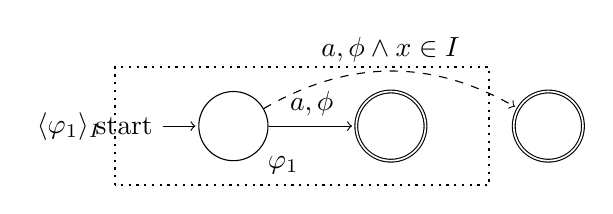
\begin{tikzpicture}[shorten >=1pt,node distance=2cm,on grid,auto]
   \draw[very thick,black](-1.5,0) node[left=1pt,fill=white]{$\langle \varphi_1  \rangle_I$};
   \draw[very thick,black](1,-0.5) node[left=1pt,fill=white]{$\varphi_1$};
   \node[state, initial] (s) {};
   \node[state, accepting] (f) [right=of s] {};
   \node[state, accepting] (f1) [right=of f] {};
   \path[->]
    (s) edge node {$a, \phi$} (f)
        edge [bend left,dashed] node {$a, \phi \wedge x\in I$} (f1);
    \draw[thick,dotted] (-1.5,-0.75) rectangle (3.25,0.75);
\end{tikzpicture}
\caption{Timed Automata from a Timed Regular Expression}
\label{fig:tretoautomata}
\end{figure}

It has been proven \cite{timedregex} that every timed regular language can be recognized by a timed automaton. We present a few simple examples of representing TREs using timed automata.

Consider the TRE $\langle \varphi_1  \rangle_I$ and its equivalent timed automaton shown in \ref{fig:tretoautomata}. Within the rectangle, we have the acceptor for $\varphi_1$ with no timing constraints. For the timed operator, a new clock $x$ is introduced and a test $x \in I$ has been added to guard every transition leading to the final state $f$.


Lets further examine the basic idea behind construction of a timed automaton for $\varphi^*$. If the time interval applies to each $\varphi$ separately, then the clocks need to be reset at each new iteration of $\varphi$. On the other hand, if the time interval applies to the whole $\varphi^*$ expression, we need the values of all clocks at each new iteration of $\varphi$ to represent the total time elapsed in the previous iterations. This is achieved by adding a new clock $x$ which is never reset to zero and transitions to the initial state in which all the clocks get the value of $x$.


\subsection{Dominant Properties}

The TRE instances generated by the binding contain every permutation of events in the alphabet within the TRE template. There is thus a total of $\Sigma^p$ possible TRE instances. Generally, we are interested in mining all of the valid TRE instances.
However, these instances contain both interesting and frequently occuring patterns, as well as those that might have been present just a handfull of times in the trace. We thus use a ranking component to reduce the mined set to contain only the dominant instances, or specifications.



\begin{defns}[Confidence]
The confidence of a TRE instance $\pi$ in a trace $t$ is the proportion of points in $t$ that do not falsify $\pi$ to the total number of points that could falsify $\pi$.
\end{defns}

\begin{defns}[Support]
The support of a TRE instance $\pi$ is the proportion of all available traces where the TRE confidence is $\ge 0$.
\end{defns}


The ranking component we use is a combination of support and confidence. The effectiveness of selecting a meaningful subset of specifications depends on picking a good set of thresholds. We express that a binding and its corresponding TRE instance are interesting if the TRE instance holds for each trace, thus $100 \%$ support. Similarly, we specify that specifications must have $ \ge 98 \%$ confidence in order to be considered dominant.

Defining a threshold for the confidence value is more difficult than for the support value. Since the total number of mined TRE instances is often very large in real systems, we would ideally keep the confidence value at $100 \%$. However, the motivation to reduce this threshold slightly is due to the presence of imperfect traces. Traces can be imperfect as a result of dropped events or execution of faulty programs. In such cases, dominant properties may not be perfectly satisfied in the collected traces. Reducing the threshold will thus include dominant properties from imperfect traces.


\section{Approach} \label{Approach}

\begin{figure}[h]
  \centering
  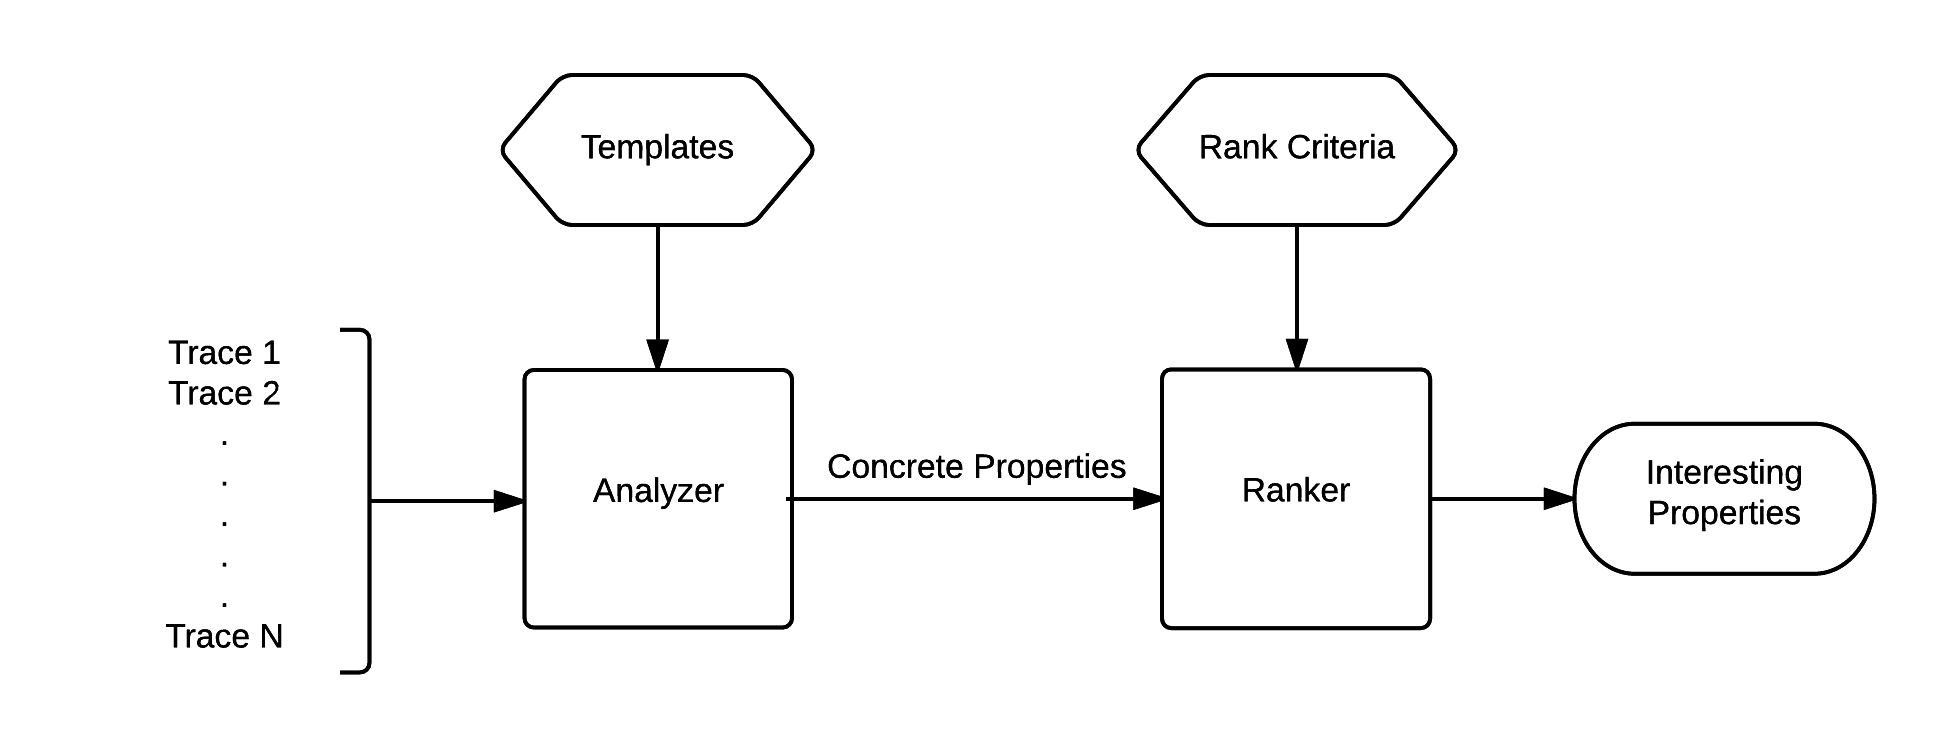
\includegraphics[trim = 1cm 0cm 0cm 0cm,clip = true,width=\linewidth]{figures/Workflow.png}
  \caption{Property Mining Workflow}
  \label{fig:work-flow Overview}
\end{figure}

% \subsection{The Workflow} \label{the_workflow}

We use execution traces collected during the runtime of a system. The event traces are generated using instrumentation already present in the system and include network traffic logs, operating system logs, or program instrumentation logs. The analyzer accepts a set of N logs, where N $\ge$ 1.

The templates in ~\ref{fig:work-flow Overview} refer to templates of temporal properties - timed regular expressions ~\cite{timedregex} that encode constraints on the relationships between subsets of trace events. Each template is an abstraction of the desired temporal property, like request, alternating, etc. ~\cite{evans1}. A template uses an abstract set of symbols ranging from $0$ to $L$, where $L$ is the length of the abstract alphabet. It also uses operators and time intervals as defined in ~\cite{timedregex}. For instance, (1.\textless0\textgreater[2,5])+ is a template for the response pattern. The '.' is the concatenation operator and the '+' is the operator for one or more instances of the expression.  The template specifies that some log event 1 is followed by another log event 0 within 2 to 5 time units, and this pattern occurs at least once in the execution trace.

The abstract alphabet is used as a placeholder. The analyzer extracts a set of S unique event symbols from the collected traces and substitutes these in place of the abstract symbols to form concrete temporal properties. In the case of (1.\textless0\textgreater[2,5])+ the analyzer will evaluate the property for all combinations of two events in S. The key insight for achieving $O(nL)$ time complexity is that an event X from the trace can be treated as either a P event or an S event.

Using an incidence matrix of dimension L we will evaluate which event combinations satisfy the given property. The acceptor FSM will iterate over the events in the system log and at each new event evaluate if any of the combinations in the matrix are satisfied. The matrix keeps track of the number of successes and failures to evaluate each concrete temporal property.


An intuitive way to evaluate a time regular expression on a system execution trace is to recursively evaluate the TRE according to its semantics on the trace. A high level description of our algorithm is presented below.


\begin{itemize}
\item \textbf{Representing a TRE} We parse the input timed regular expression and transform it into a timed automata.
\item \textbf{Representing a trace} We parse the input trace into a  linear array representation where each unique event has its corresponding time and event id [time, eventid].
\item \textbf{Checking property instances over traces} We iterate over the set of each unique event and process the entire trace with respect to each unique event. Updating the \emph{success} and \emph{reset} for the entire trace. Processing the trace refers to matching the required TRE in the process trace.
\end{itemize}


\begin{algorithm}[h]
    \caption{Timed Regular Expression Mining}\label{alg:the_alg}
    \begin{algorithmic}[1]
     \Require  Given a set of traces with unique event \emph{i} and a TRE pattern
     \Ensure Parse TRE and formulate a finite Timed Automaton $\rightarrow$ A
     \State Initialize the incidence matrix of size $\Sigma^p$
     \State Initialize the \emph{success} and \emph{reset} counters for all permutations
     \For {(each unique event $i$ from the trace)}
        \State Process the complete trace;
        \State Update the success if A $\rightarrow$ FS;
        \State Update the reset if A $\rightarrow$ ES;
     \EndFor
     \State Evaluate Support - S
     \State Evaluate Confidence - C
    \end{algorithmic}
\end{algorithm}

In Algorithm ~\ref{alg:the_alg} $\Sigma$ is the set of alphabets and $p$ is the number of place holders in the TRE. $A$ denotes the timed automaton and $FS$ and $ES$ denote the final and error states of the timed automaton. $S$ and $C$ denote the \emph{support} and \emph{confidence} metrics of the TRE on the given trace.

We used the most commonly occurring temporal property patterns \cite{evans} by transforming them into Time Regular Temporal Property patterns. Let us assume we have several causing events $P$ to share one effect event $S$. The TRE property patterns are presented in Table ~\ref{TRE_Exp}.
\begin{table}[ht]
  \centering
  \begin{tabular}{|c|c|}
  \hline
  % after \\: \hline or \cline{col1-col2} \cline{col3-col4} ...
  \textbf{Name} & \textbf{TRE}  \\ \hline
  Response      & $[-P]^*;((P;[-S]^*;S \langle x,y \rangle);[-P]^*)^*$        \\ \hline
  Alternating   & $[-P,S]^*;(P;[-P,S]^*;S;[-P,S]^* \langle x,y \rangle)^*$       \\ \hline
  MultiEffect   &  $[-P,S]^*;(P;[-P,S]^*;S;[-P]^* \langle x,y \rangle)^*$     \\ \hline
  MutiCause     &  $[-P,S]^*;(P;[-S]^*;S;[-P,S]^* \langle x,y \rangle)^*$     \\ \hline
  EffectFirst   &  $[-P]^*;(P;[-P,S]^*;S;[-P,S]^* \langle x,y \rangle)^*$      \\ \hline
  CauseFirst    &  $[-P,S]^*;(P;[-S]^*;S;\langle x,y \rangle [-P]^*)^*$       \\ \hline
  OneCause      &  $[-P]^*;(P;[-P,S]^*;S;\langle x,y \rangle [-P]^*)^*$       \\ \hline
  OneEffect     &  $[-P]^*;(P;[-S]^*;S;[-P,S]^* \langle x,y \rangle)^*$       \\ \hline
\end{tabular}
\caption{TRE Property Patterns}\label{TRE_Exp}
\end{table}


\section{Evaluation}
%% author: YJ
In this Section, we demonstrate the performance, scalability and usefulness of our approach. Our code is implemented as an R package\footnote{\url{https://github.com/gretac/ura.git}}, which internally uses C++ code for performance. `Rcpp'\footnote{\url{http://www.rcpp.org/}} is used for integration of R and  C++ modules. Ragel\footnote{\url{http://www.colm.net/open-source/ragel/}} is used to synthesize Timed Automata for TREs. We developed TRE variants of commonly used patterns of QREs~\cite{DBLP:conf/paste/YangE04}. By using these TRE variants as TRE templates, we mined TRE instances from real-world datasets: QNX traces and traces from controller area network (CAN). We used different thresholds for \emph{support} and \emph{confidence} to uncover interesting TRE instances. Further, to demonstrate the performance and scalability of our approach, we synthesized traces for different configurations w.r.t. the length of traces, number of variables in a TRE template and the number of distinct events in traces. For the experiments, we used a single eight core machine equipped with the Intel i7-3820 CPU at 3.60GHz and 31.4Gb of RAM. The machine runs Ubuntu 14.04 LTS 64 bit.

\subsection{Performance Evaluation using Synthesized Traces}
We synthesized traces by varying the following three parameters for execution traces: distinct number of events, total number of events and the number of variables in TRE templates. We used TREs in following classes of timed variants of commonly used property patterns: response, alternating, multi-effect, mutli-cause, effect-first, cause-first, one-cause and one-effect. We evaluated the performance of our mining algorithm under three different setups in which the value of one of the three parameters is varied by keeping the values of other parameters as constants.

\todo[inline]{By Yogi: Add reference to loop in algorithm section}
\noindent \textbf{Settings and Results:} We performed the experiment under four different settings. In each of the settings, the value of one of the parameters was varied. The values of others were kept constant. We executed each experiment 10 times.

\noindent \textbf{Setting 1:}
In Setting 1, the total number of events in execution traces were varied. The number of distinct events was set to 4, and the number of variables in TRE templates is set to 2. The details of four TRE templates, used in this experiment, are provided further in this section. The total number of events in execution traces were varied exponentially. As shown in Figure~\ref{fig:plot1}, the x axis shows the total number of events in execution traces, and the y axis shows the average overhead of our mining algorithm in terms of execution time. We note that we begin to measure the overhead of our algorithm when individual events are processed in the loop . Thus, the measurement does not include the initialization part of the algorithm whose overhead is constant. As shown in Figure~\ref{fig:plot1}, the overhead of our mining algorithms grows linearly w.r.t. the total number of events in a execution trace. For example, the average execution time is 170 milliseconds for processing 0.1 million events.

\noindent \textbf{Setting 2:}
In Setting 2, the number of distinct events is varied. There were 10,000 events in each execution trace, and the number of variables in TRE templates were set to 2. As shown in Figure~\ref{fig:plot2}, the x axis shows the number of distinct events in execution traces. The y axis reports the execution time of the mining algorithm. As seen, the overhead increases exponentially. The average overhead for processing a trace of 10,000 events with 25 distinct events is 594 milliseconds.

We used the following TRE templates for Setting 1 and Setting 2.

\noindent \textbf{T-1 (response)}: $(\verb!^!P)^*.((\langle P.(\verb!^!S)^*.S\rangle[0, 2000]).(\verb!^!P)^*$

\noindent \textbf{T-2 (alternating)}: $(\verb!^!P,S)^*.((\langle P.(\verb!^!P,S)^*.S\rangle[0, 2000]).(\verb!^!P,S)^*$

\noindent \textbf{T-3 (multi-effect)}: $(\verb!^!P,S)^*.((\langle P.(\verb!^!P,S)^*.S\rangle[0, 2000]).(\verb!^!P)^*$

\noindent \textbf{T-4 (multi-cause)}: $(\verb!^!P,S)^*.((\langle P.(\verb!^!S)^*.S\rangle[0, 2000]).(\verb!^!P,S)^*$

\noindent \textbf{Setting 3:}
In Setting 3, we varied the number of parameters in TRE templates. The total number of events in execution traces were set constant at 10,000, and the number of distinct events was set to 10. Figure~\ref{fig:plot3} shows the variation in the average overhead w.r.t. the number of variables in TRE templates. As shown, the average overhead grows exponentially. The average overhead for processing an execution trace of 10,000 events with 10 distinct events with a TRE template containing 4 variables is 4156 milliseconds. For this setting, we used TRE templates with different number of variables, which are similar to the TRE templates used for Setting 1 and Setting 2. For the sake of brevity, we do not list these TRE templates.

The experimental results confirm the asymptotic analysis of our algorithm's complexity, which is described in previous sections.

We also compared the performance of Algorithm 1 and Algorithm 2 over synthesized traces. The size of the execution trace for this experiment was 50,000, and 30 distinct types of events were used. The following TRE templates were provided as an input to the algorithms.

\begin{table*}[t]
	\centering
	\begin{tabular}{|l|l|}
		\hline
		\textbf{TRE templates for Algorithm 1} & \textbf{TRE templates for Algorithm 2} \\
		\hline
		 $(\langle P.\verb!^!Q^*.Q.\verb!^!R^*.R \rangle [1, 5000])$& $(\langle P.Q.R \rangle [1, 5000])$ \\
	\end{tabular}

	\caption{Comparing Algorithm 1 and Algorithm 2}
	\label{miningOverhead}
\end{table*}

\begin{figure*}
  \centering
  \subfloat[Varying total number of events]{
  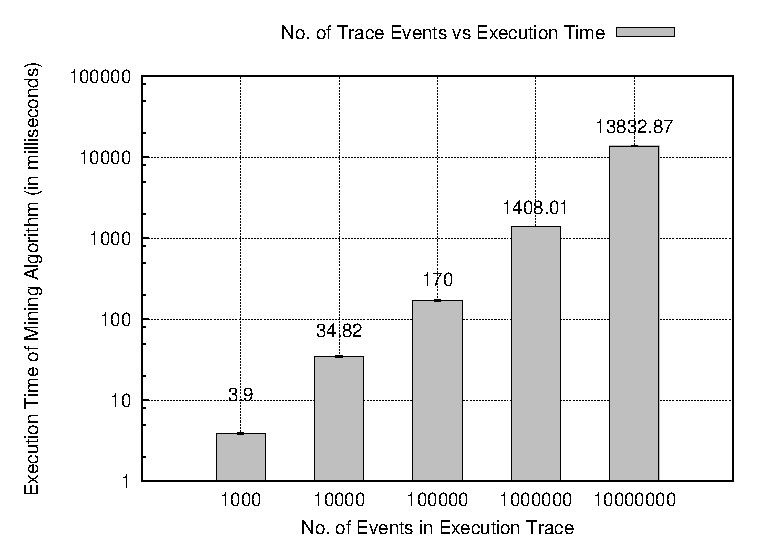
\includegraphics[width=\columnwidth]{Plot1.eps}
  \label{fig:plot1}
  }
  \subfloat[Varying number of distinct events]{
  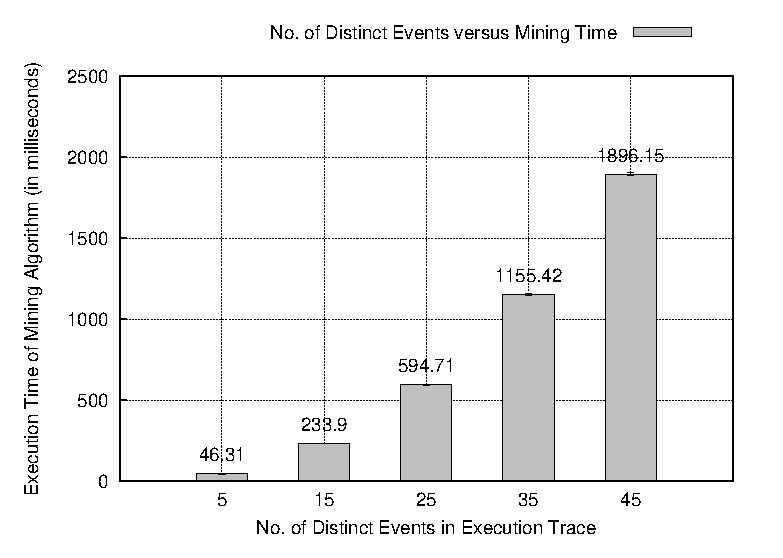
\includegraphics[width=\columnwidth]{Plot2.eps}
  \label{fig:plot2}
  }\\
  \subfloat[Varying number of variables in TRE templates]{
  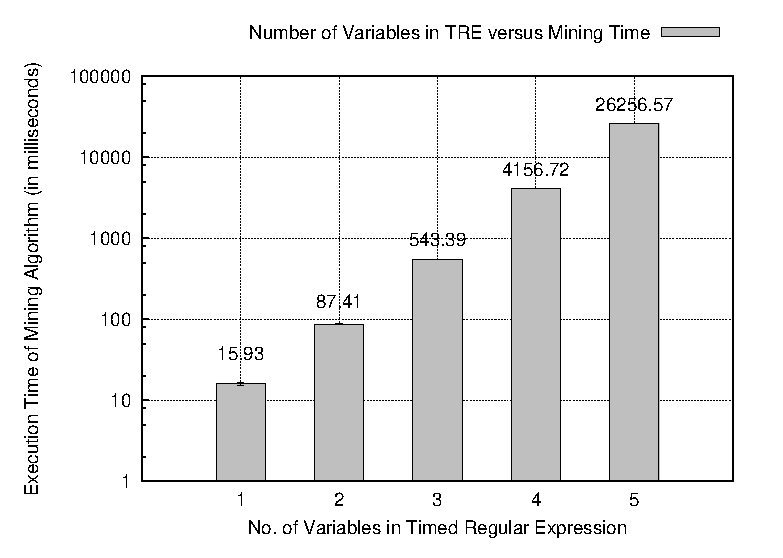
\includegraphics[width=\columnwidth]{Plot3.eps}
  \label{fig:plot3}
  }
  \subfloat[Comparing Overhead of Mining Different Classes of TRE templates]{
  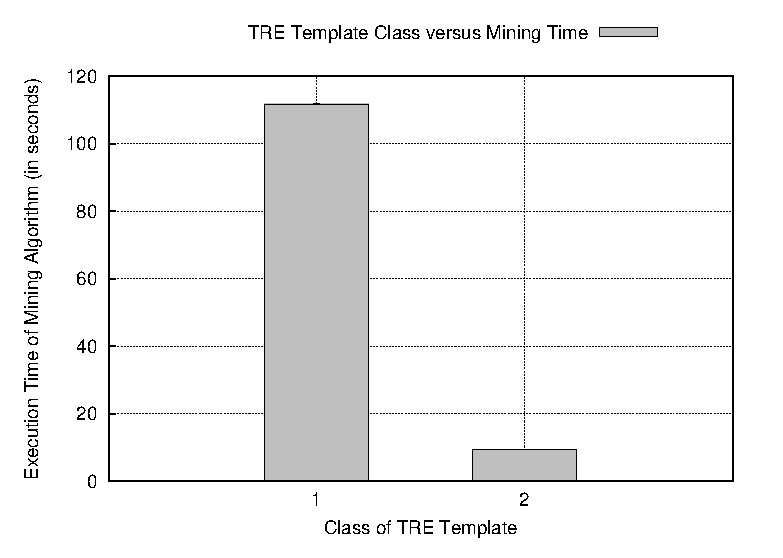
\includegraphics[width=\columnwidth]{Plot4.eps}
  \label{fig:plot4}}
  \caption{Results on Synthesized Traces}
\end{figure*}


\section{Discussion} \label{discussion}

The following discussion examines the following important characteristics of the technique we presented in this paper for mining temporal properties in the form of TREs from traces: soundness, completeness, optimality (in terms of space and runtime), and scalability.


\subsection{Sound and Complete}

%% talk about the technique being sound and complete

% We also prove that our technique is sound, i.e., a mined specification reported by our algorithms actually satisfies the given thresholds of support and confidence on the provided input traces. Also, our technique is complete, i.e., our algorithms report all TRE instances which comply on given traces w.r.t. the thresholds of support and confidence.

First we can look at regular expressions and their acceptors without the timing constraints. Regular expressions offer a declarative way to express the patterns that we want to accept. Every language defined by a regular expression is also defined by a finite automaton, as defined by Theorem 3.7 in ~\cite{book1}. There is a way to convert any regular expression into a non-deterministic automaton, and further to convert from a non-deterministic to a deterministic automaton. We can thus generate a Deterministic Finite Automaton (DFA) for any regular expression.

Similarly, timed automata are recognizers of timed languages. They have states, as any FSM, as well as clocks. Every timed language defined by a (generalized extended) regular expression is accepted by a timed automaton, as defined by Theorem 2 in ~\cite{timedregex}. Thus, timed automata and generalized timed regular expressions have the same expressive power.

The language of a timed automaton consists of all the strings that it accepts ~\cite{timedregex}. The strings in our case are sequences of time-event pairs. The timed automata we generate are acceptors for strings that satisfy the desired property. The more strings in the trace that can be accepted, the more dominant is the property.

\subsection{Memory Requirements}

Our property mining technique requires space for storing the multidimensional results matrix, the FSM, and
the trace itself.

The storage requirements for the matrix are directly influenced by $p$ and $\Sigma$.
We want to encode the matrix to hold the evaluation results of every combination of unique events that fit in the TRE.
Thus we need $O(\Sigma^p)$ space to hold the acceptor results.

The dimensionality of the matrix grows proportionally to $p$, the number of symbols in the desired property.
Complex properties that encode a relationship between a large number of events will result in higehr values of $p$.
Increasing values of $p$ result in exponential space growth.
However, the majority of properties of interest represent relationships among a few events only ~\cite{evans1, dwyer1999patterns}.
Thus, in general, the dimension $p$ of the matrix will remain small.
According to the properties listed in ~\cite{dwyer1999patterns, dwyer2}, the typical property will be constrained to 6 events.

The value of $\Sigma$, on the other hand, affects the size of each dimension.
The number of unique events $\Sigma$ in the trace will depend on the complexity of the program or system.
However $\Sigma$ has a much smaller effect on the growth of the matrix since it only affects the base number in the
exponential space complexity.


Next, we consider the storage requirements for the FSM used to evaluate the TRE.
The storage required for the FSM is proportional to the number of its states ~\cite{book1}.
If $n$ is the length of the TRE, then an equivalent NFA has $O(n)$ states
and an equivalent DFA has at most $O(\Sigma^n)$ states. Similar to the matrix, complex properties that encode a lot of relationships between events result in exponential space growth for the FSM. However, majority of interesting properties will remain simple ~\cite{dwyer1999patterns}.


Lastly, the storage requirements for the trace are equivalent to the length of the trace, $O(L)$.
Our mining approach examines one time event pair from the trace at a time, without needing to
store any past or future events for context. It also does not perform any changes on the
contents of the trace. Thus the trace is stored only once and never replicated.

%% Discuss optimality & scalability


\subsubsection{Runtime Requirements}

We assess the performance of our mining approach in terms of the time required to evalute a TRE template on a set of collected system traces.

The runtime performance of the proposed technique differs depending on whether negation is included within the expression.
Lets first consider the runtime with negation. When an event variable in the TRE template is negated, the automaton must evaluate all existing TRE instances. This is bacause at evaluation time the satisfiability of any of the TRE instance may be affected. The automaton will thus evaluate $O(\Sigma^p)$ TRE instances for every time-event pair in the trace. Given that the length of the trace $t$ is $L$, the overall runtime will be $O(\Sigma^p \times L)$.

Next we will consider the runtime of the techinique for TRE templates without negation. This case differs in that only the TRE instances where the bounded event corresponds to that read from the trace needs to be evaluated. We can thus reduce the previous runtime by evaluating ony a subset of all TRE instances. Providing a bound on the runtime relies on an analysis of the subset of TRE instances that contain the observed event.

Considering that the binding function maps events to event variables with no replacement, meaning different events canot be mapped to the same event variable, there will be $p \times ^{(\Sigma - 1)}P_{(p - 1)}$ TRE instances that will need to be evaluated. This is equivalent to $\frac{p \times (\Sigma - 1)!}{(\Sigma - p)!}$. The overall runtime without negation is thus
$O(p \times ^{(\Sigma - 1)}P_{(p - 1)} \times L)$. The relative speedup when compared to the runtime for expressions with negation is $\frac{\Sigma}{p}$.

%% Discuss optimality & scalability

Generally, scalability of dynamic property mining techniques is limited.
The techniques tend to scale poorly with the size of the input trace $L$. Our technique is optimal in that respect as the runtime grows linearly with the increasing size of $L$. Given that $L \gg \Sigma$ and $L \gg p$, reading each line of the trace at most once is preffered.

Finally, as mentioned earlier, since the majority of interesting properties are not complex, $\Sigma^p$ will remain small in majority of real life situations.


\section{Conclusion}

TBD


%\bibliographystyle{abbrv}
\bibliographystyle{plainnat}
\bibliography{refs}


\end{document}
